\documentclass[11pt]{article}
\usepackage{amsmath,graphicx,booktabs,geometry,hyperref}
\geometry{margin=22mm}
\title{Verification of Full Collocated SIMPLE on Conforming Curved Meshes and CPU/CUDA Execution}
\author{TensorFVM benchmark development}
\begin{document}\maketitle
\begin{abstract}
A continuous manufactured incompressible Navier--Stokes problem tests full momentum, pressure correction and nonorthogonal geometry. A separate fully turbulent Spalart--Allmaras plate tests steady convergence and device equivalence. All failures and independent physical gates are retained.
\end{abstract}
\section{Problem}
Let $g(x)=0.2\sin^4(\pi x/2)$, $0\leq x\leq2$, $g(x)\leq y\leq g(x)+1$.
With $\eta=y-g(x)$, $w=6\eta(1-\eta)$, prescribe
$\mathbf{u}=(w,g'w)$ and $p=12\mu(2-x)$.
The forcing is $\mathbf{f}=\rho(\mathbf{u}\cdot\nabla)\mathbf{u}+\nabla p-\mu\Delta\mathbf{u}$.
Both velocity components and pressure are numerically solved; analytic fields are used only for forcing/boundaries and error evaluation. Refined starts interpolate computed coarse solutions.
\section{Method and acceptance}
Production collocated SIMPLE, Rhie--Chow face flux, upwind momentum convection and nonorthogonal diffusion use conforming polygons. Optional sparse GMRES has true residual checks and line/coarse pressure preconditioning. Host CSR assembly and transfer are explicit; Krylov iterations and preconditioning execute on actual CPU/CUDA. A coupled coarse Picard residual correction accelerates fine-grid SIMPLE. Interpolation and coarse updates use a constant-mobility auxiliary velocity projection while retaining physical pressure. The final physical Rhie--Chow flux defect must be below $10^{-7}$. Boundary faces are polygon chords sampled on the curve. SA has up to eight transport subiterations. Every physical error gate is strictly below 3\%; steady residual and device equivalence are separate. SA empirical mean skin friction is not an exact DNS reference.
\section{Timing}
CPU is single-threaded, float64; CUDA is RTX3090. Complete CPU/CUDA steady solves are performed once each. Three warmed synchronized five-step windows from the same computed intermediate state are reported separately and include assembly and transfer, excluding restore and plotting. Window ratios must not be presented as complete solve speedups.
\section{Results}
\begin{tabular}{lrrrr}\toprule Case & Cells & Velocity L2 (\%) & Pressure L2 (\%) & Window CPU/CUDA\\\midrule
curved-32x16 & 512 & 0.420476 & 0.847160 & 0.678 \\
curved-64x32 & 2048 & 0.159306 & 0.199764 & 1.059 \\
curved-128x64 & 8192 & 0.074600 & 0.061110 & 1.985 \\
curved-256x128 & 32768 & 0.037391 & 0.029793 & 3.877 \\
sa-64x56 & 3584 & -- & -- & 1.269 \\
\bottomrule\end{tabular}
\section{Fields, curves and convergence}
\begin{figure}[p]\centering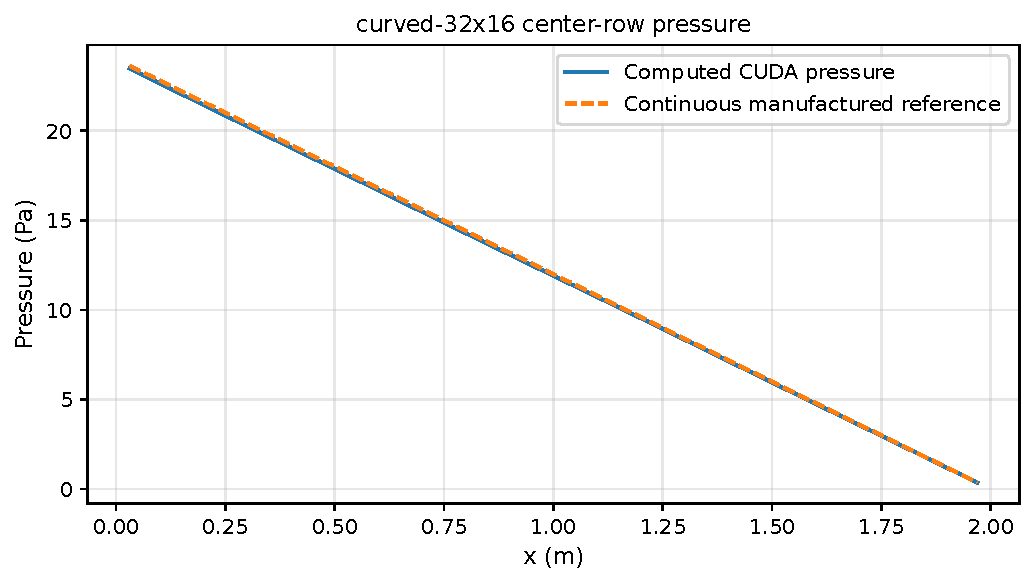
\includegraphics[width=.9\linewidth]{figures/curved-32x16-pressure-curve.pdf}\caption{curved 32x16 pressure curve}\end{figure}
\begin{figure}[p]\centering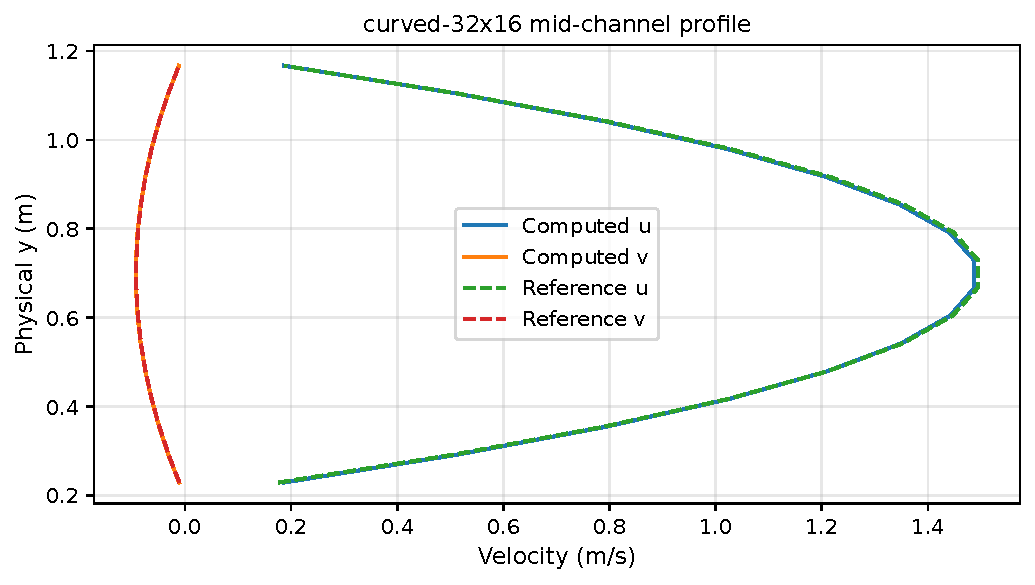
\includegraphics[width=.9\linewidth]{figures/curved-32x16-velocity-profile.pdf}\caption{curved 32x16 velocity profile}\end{figure}
\begin{figure}[p]\centering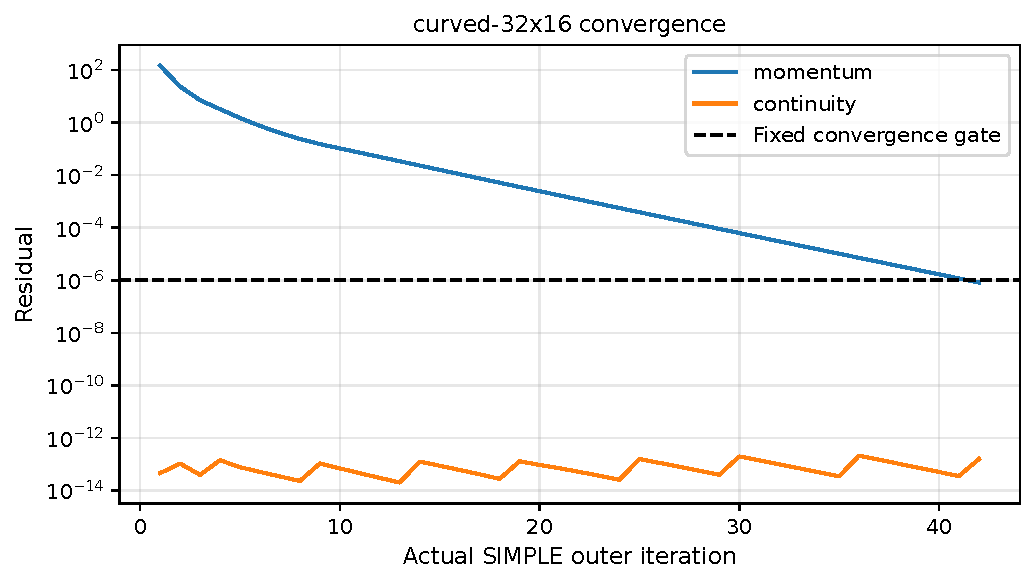
\includegraphics[width=.9\linewidth]{figures/curved-32x16-residuals.pdf}\caption{curved 32x16 residuals}\end{figure}
\begin{figure}[p]\centering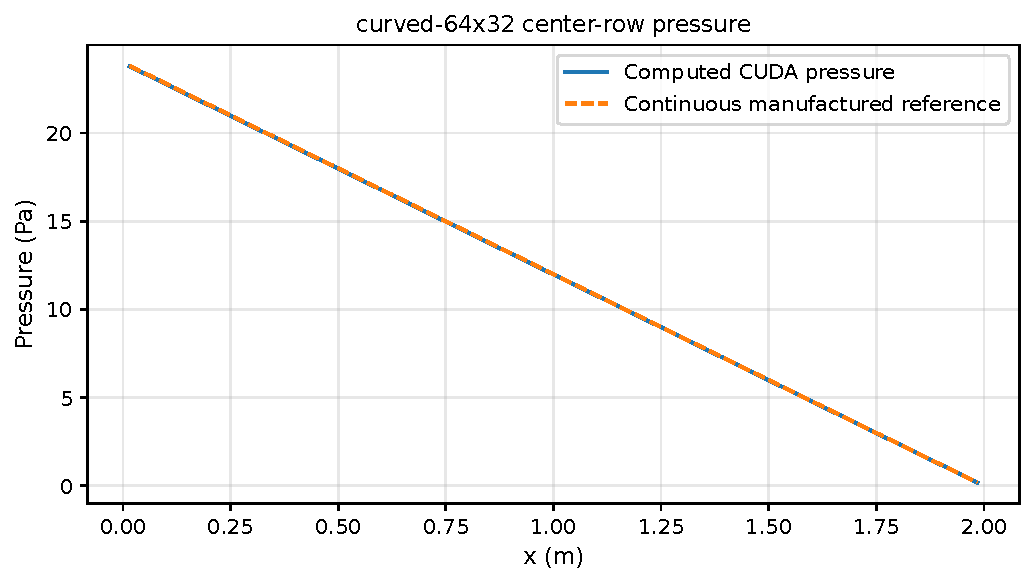
\includegraphics[width=.9\linewidth]{figures/curved-64x32-pressure-curve.pdf}\caption{curved 64x32 pressure curve}\end{figure}
\begin{figure}[p]\centering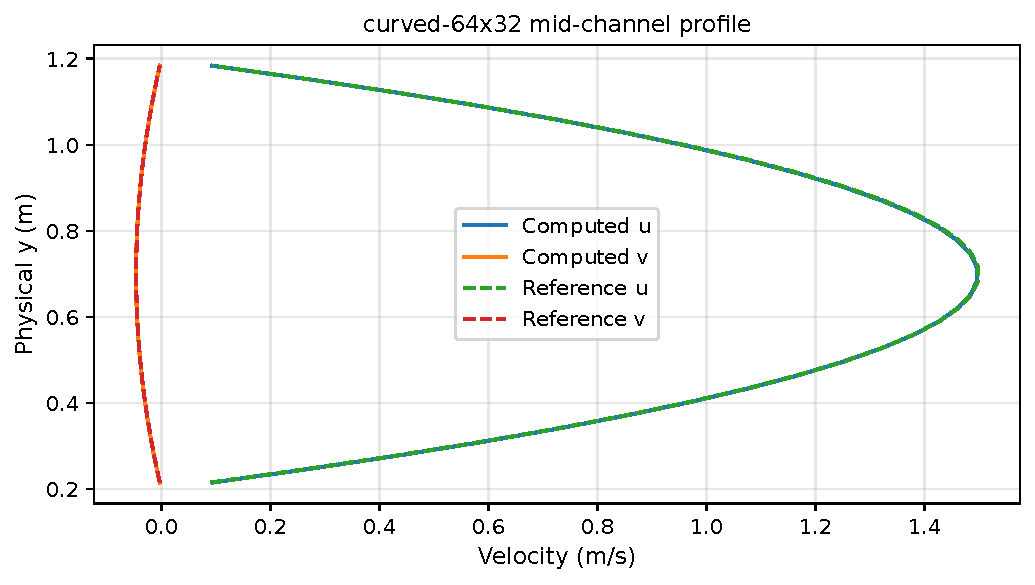
\includegraphics[width=.9\linewidth]{figures/curved-64x32-velocity-profile.pdf}\caption{curved 64x32 velocity profile}\end{figure}
\begin{figure}[p]\centering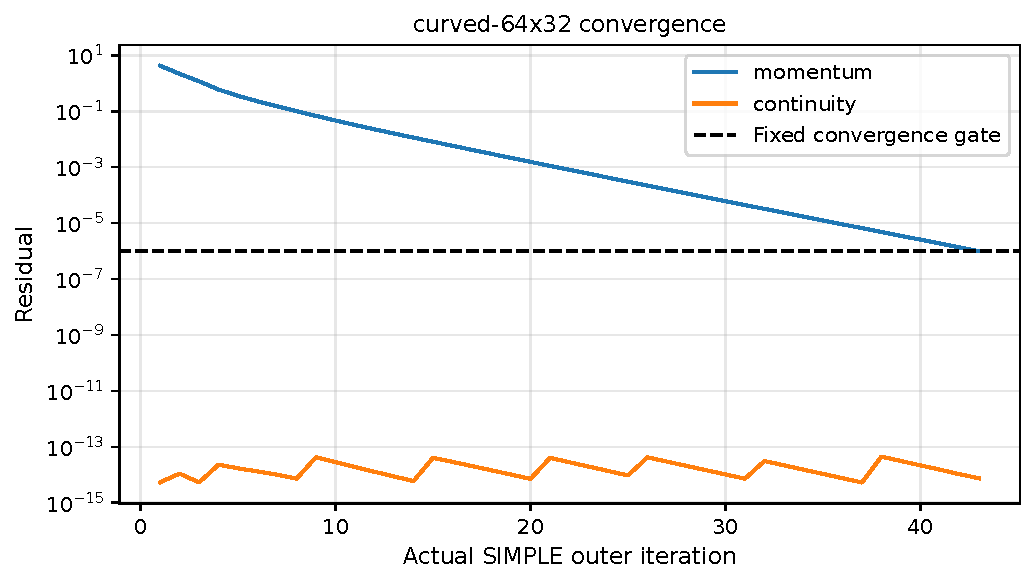
\includegraphics[width=.9\linewidth]{figures/curved-64x32-residuals.pdf}\caption{curved 64x32 residuals}\end{figure}
\begin{figure}[p]\centering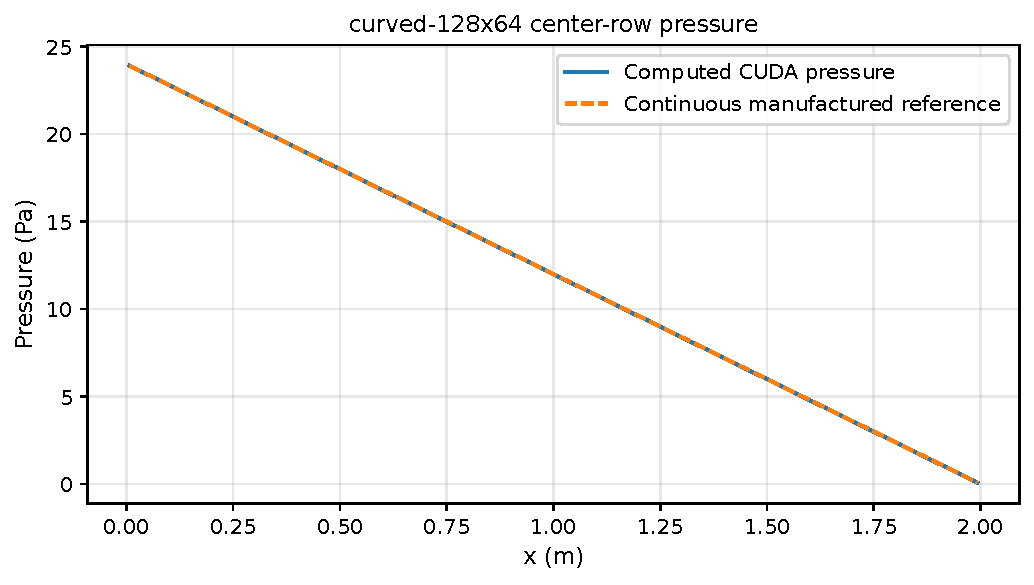
\includegraphics[width=.9\linewidth]{figures/curved-128x64-pressure-curve.pdf}\caption{curved 128x64 pressure curve}\end{figure}
\begin{figure}[p]\centering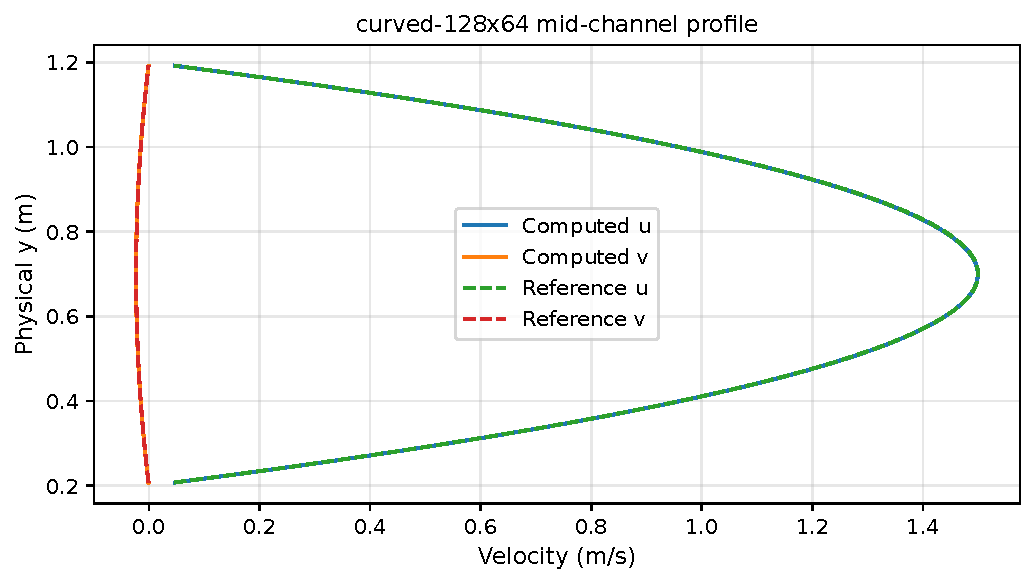
\includegraphics[width=.9\linewidth]{figures/curved-128x64-velocity-profile.pdf}\caption{curved 128x64 velocity profile}\end{figure}
\begin{figure}[p]\centering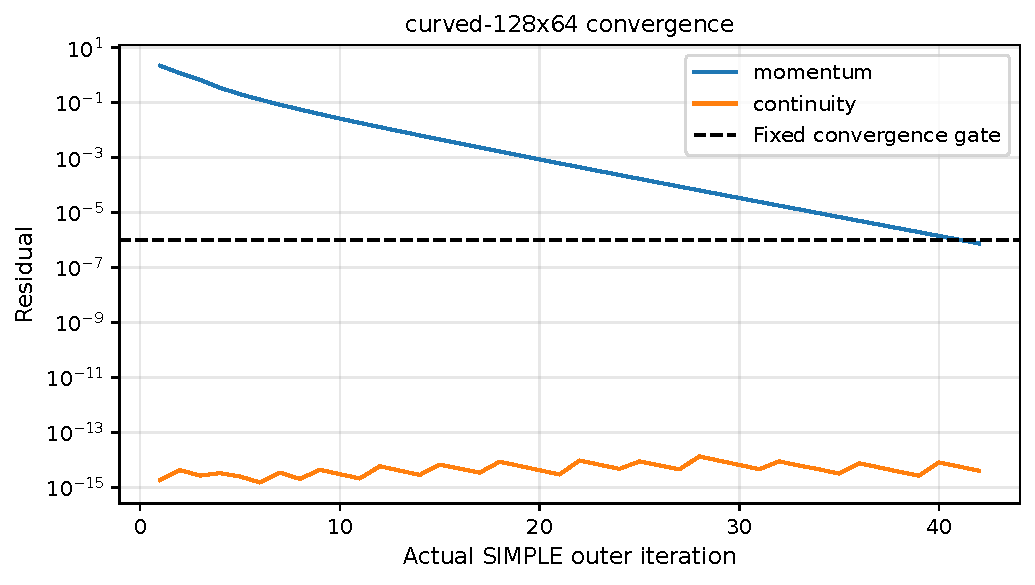
\includegraphics[width=.9\linewidth]{figures/curved-128x64-residuals.pdf}\caption{curved 128x64 residuals}\end{figure}
\begin{figure}[p]\centering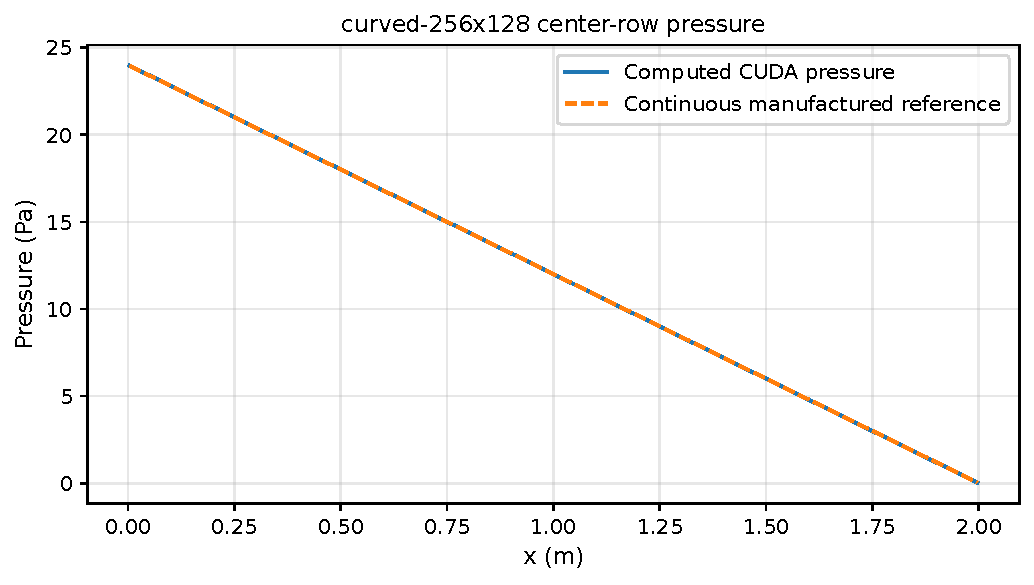
\includegraphics[width=.9\linewidth]{figures/curved-256x128-pressure-curve.pdf}\caption{curved 256x128 pressure curve}\end{figure}
\begin{figure}[p]\centering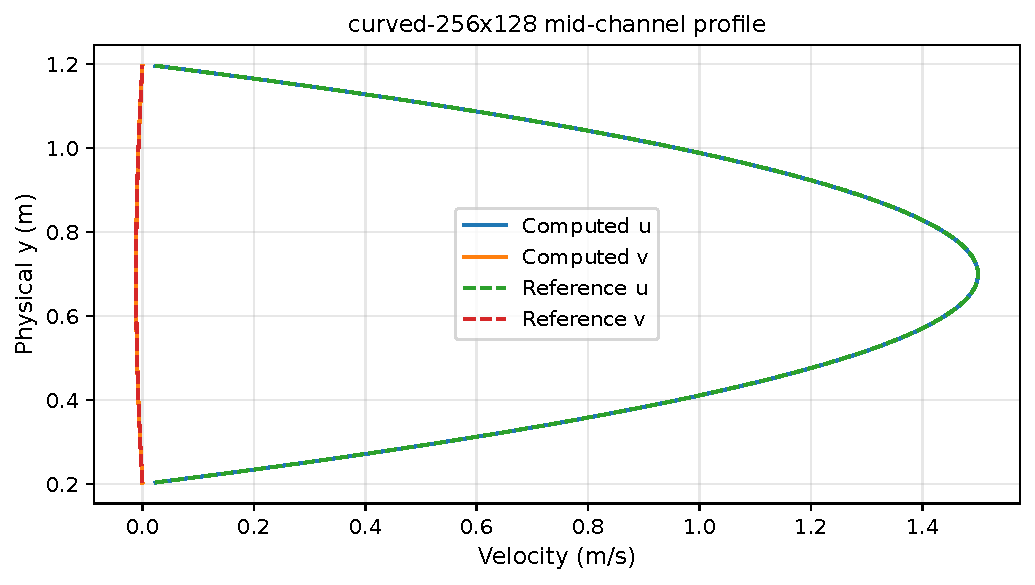
\includegraphics[width=.9\linewidth]{figures/curved-256x128-velocity-profile.pdf}\caption{curved 256x128 velocity profile}\end{figure}
\begin{figure}[p]\centering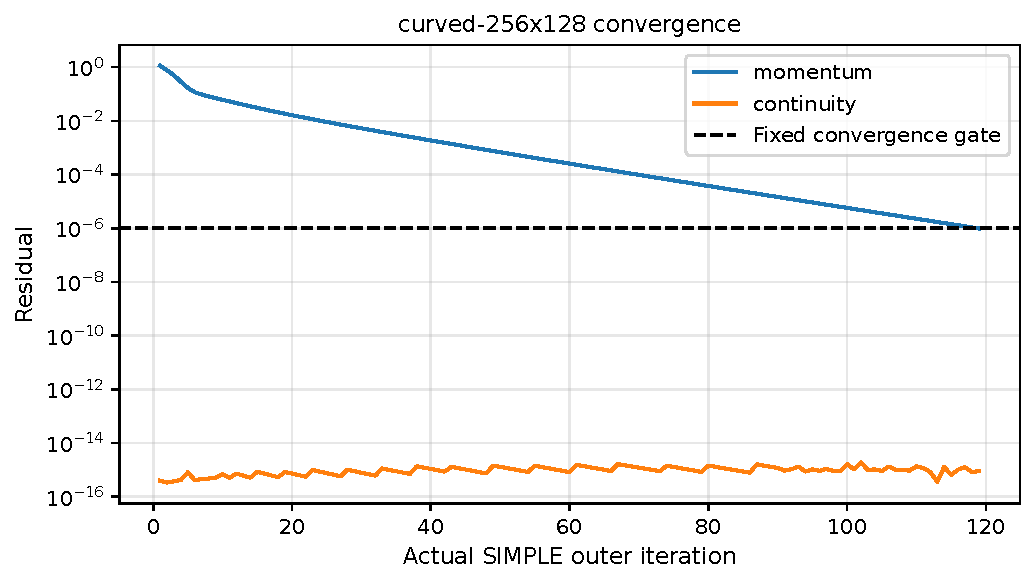
\includegraphics[width=.9\linewidth]{figures/curved-256x128-residuals.pdf}\caption{curved 256x128 residuals}\end{figure}
\begin{figure}[p]\centering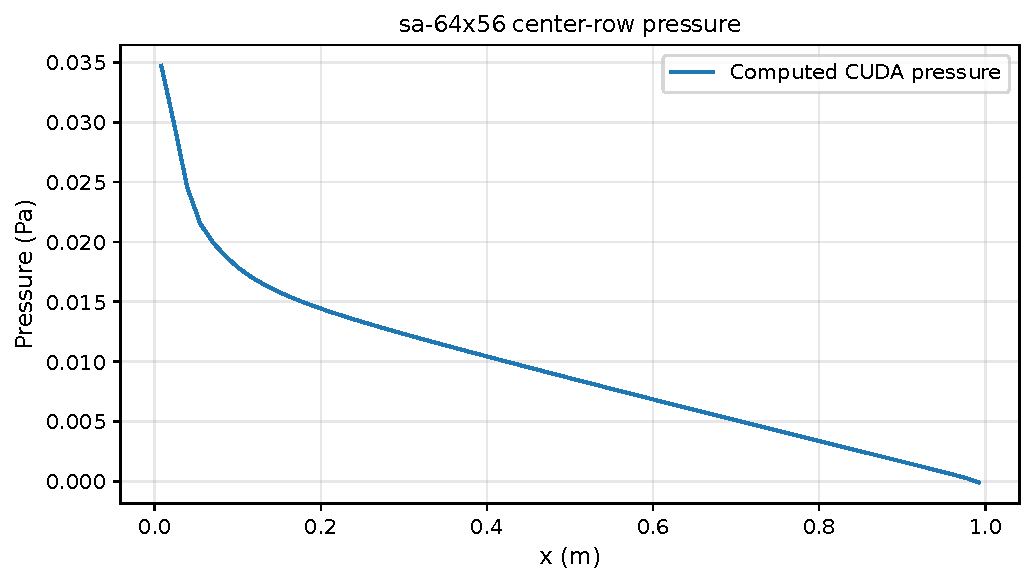
\includegraphics[width=.9\linewidth]{figures/sa-64x56-pressure-curve.pdf}\caption{sa 64x56 pressure curve}\end{figure}
\begin{figure}[p]\centering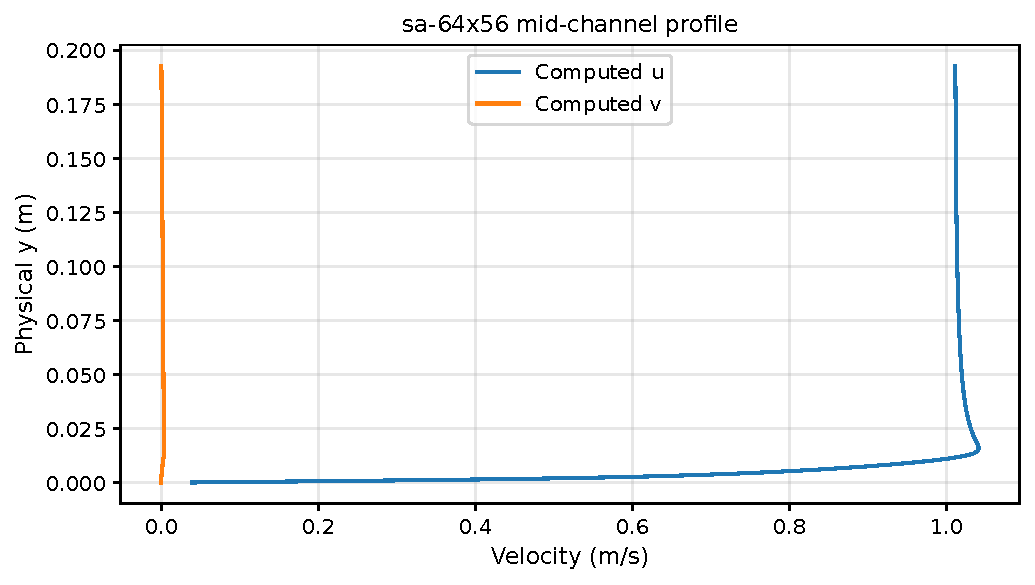
\includegraphics[width=.9\linewidth]{figures/sa-64x56-velocity-profile.pdf}\caption{sa 64x56 velocity profile}\end{figure}
\begin{figure}[p]\centering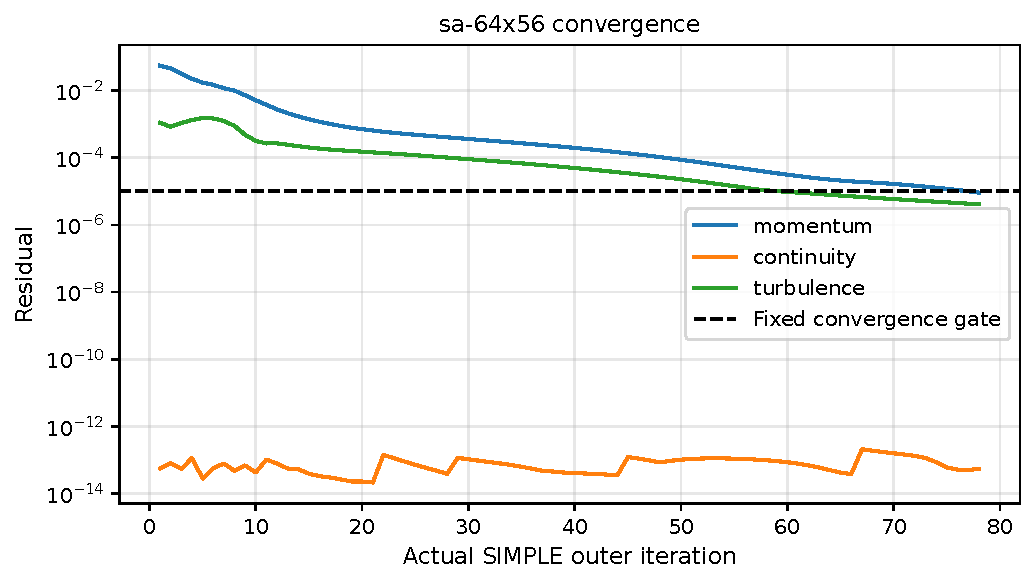
\includegraphics[width=.9\linewidth]{figures/sa-64x56-residuals.pdf}\caption{sa 64x56 residuals}\end{figure}
\begin{figure}[p]\centering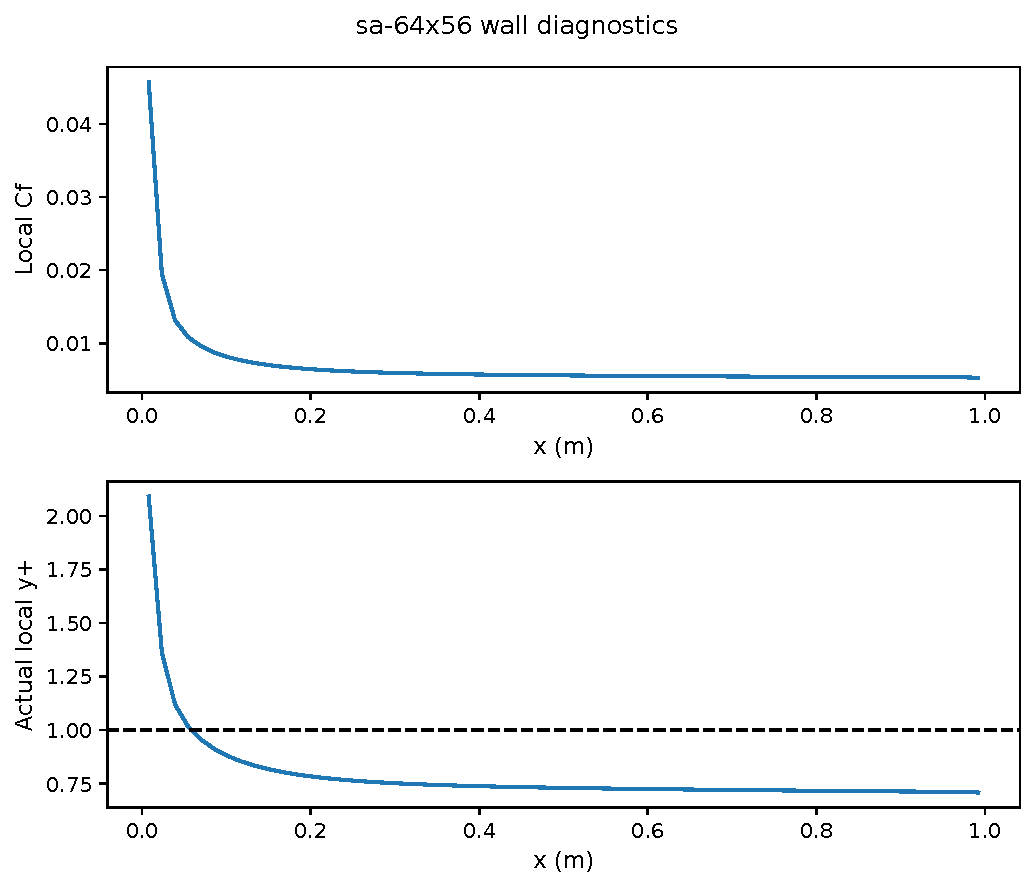
\includegraphics[width=.9\linewidth]{figures/sa-64x56-cf-yplus.pdf}\caption{sa 64x56 cf yplus}\end{figure}
\section{Scope} This two-dimensional manufactured curved channel is not an unforced bend or an industrial SUBOFF validation. Steady SA, device consistency and empirical skin-friction accuracy remain separate statements. SIMPLEC, PISO and PIMPLE are not implemented in this delivery.\end{document}
